\chapter{Fundamentals II}
\label{cha:Fundamentals II}

This chapter provides an overview of foundational concepts relevant to the thesis. It begins by reviewing various positioning methods as well as systems for indoor and outdoor settings, followed by an examination of how smartphones handle alerts, including different types and influencing factors in iOS. Geofencing technologies are analyzed for their functionality, use cases and limitations. Finally, advancements in technologies such as speech-to-text and large language models are discussed in the context of voice-controlled reminder systems.

\section{Positioning Methods}
The term "positioning" refers to the ability to determine an object's location within a defined space. According to K\"upper \cite{kupper2005location}, positioning relies on the measurement of observables, which describe the spatial relationship between a target and its reference points. Depending on the positioning technology used, observables can include angles, ranges, range differences or velocity and they are measured by analyzing the properties of pilot signals. 
Pilot signals, such as radio, infrared or ultrasound signals, are reference signals transmitted from a known source and by identifying their origin—a fixed point with known coordinates—the position of the target can be calculated using positioning techniques. These techniques vary based on the type of observable measured and include proximity sensing, lateration, angulation, pattern matching and inertial navigation.
The computed position is expressed relative to a chosen reference system. This system could be descriptive, such as identifying a specific cell in a grid, or geodetic, where the position is represented as two- or three-dimensional coordinates in systems like WGS-84. Further details on the different positioning techniques are provided in the following sections.

\subsection{Proximity Sensing}
Proximity sensing, as described by K\"upper \cite{kupper2005location}, is the simplest positioning method.
It works by leveraging the limited coverage range of pilot signals to detect the presence or absence of a terminal within a specific area. 
In this context, a terminal refers to a device or object whose position is being determined, such as a mobile or IoT device.
Due to the limited range of these pilot signals, the terminal's position is assumed to correspond to the location of the base station communicating with it.
Militaru et al. \cite{militaru2024positioning} illustrate the concept of proximity sensing in Fig.~\ref{fig:proximity2}.

\begin{figure}[htbp]
    \centering
    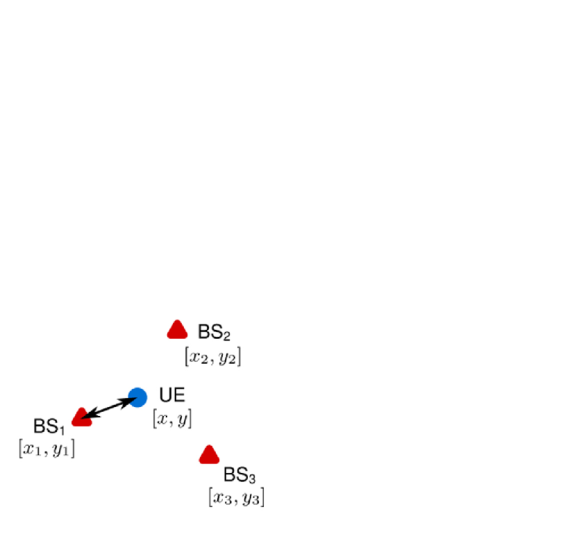
\includegraphics[width=0.4\textwidth]{proximity2.pdf}
    \caption{Proximity sensing \cite{militaru2024positioning}}
    \label{fig:proximity2}
\end{figure}

In the words of K\"upper \cite{kupper2005location}, proximity sensing in cellular networks is often referred to as Cell of Origin (CoO), Cell Global Identity or Cell-ID. 
A "cell" is a geographic area within the cellular network, managed by a base station that serves as a local signal hub for devices within that area. 
The accuracy of the location determined through CoO depends largely on the size and shape of the cell, as highlighted by Grejner-Brzezinska and Kealy \cite{grejner2004positioning} and Lee et al. \cite{lee2014localization}.
Smaller cells allow for better location estimates, often reaching accuracy within 100 meters in urban areas where cell towers are densely placed. However, as the density of cells increases, the computational cost of this method also rises.
In rural areas, where cell coverage spans several kilometers, the location estimate becomes less accurate.

CoO is considered an inexpensive solution, as noted by Grejner-Brzezinska and Kealy \cite{grejner2004positioning}, because it is compatible with the existing infrastructure. 
A terminal can determine its location using CoO either through an active connection to a base station or by passively receiving broadcast signals while in an idle state. 
When actively connected, the terminal's location is identified using the coordinates of the serving base station. 
In idle mode, the terminal can either query a remote database to retrieve the base station's location using its cell ID or rely on the base station to include its location directly in the broadcast signal, reducing the need for external lookups. 

\subsection{Lateration}
Lateration, the most widely used method for localization according to Lee et al. \cite{lee2014localization}, determines a target's location by measuring distances or distance differences from multiple reference stations. 
These measurements are referred to as "pseudoranges" because they include errors that distort the true ranges. 
Common error sources in lateration include clock errors, atmospheric effects or multipath propagation.
To determine a position fix, measurements from at least three stations are required.
Lateration techniques are categorized into circular lateration, which relies on absolute distance measurements and hyperbolic lateration, which uses differences in these distances across stations.

\subsubsection{Circular Lateration}
Circular lateration uses distance measurements to multiple base stations to derive a location. Assuming the base stations are at the same elevation, knowing the distance between the target and a single base station places the target somewhere on a circle centered on that station. Introducing a second base station allows for two possible positions where the two circles intersect. Adding a third base station resolves this uncertainty, pinpointing the target's exact location at the single intersection point of all three circles, according to K\"upper \cite{kupper2005location}. This process, known as trilateration, utilizes the Pythagorean theorem for calculations and is illustrated in Fig.~\ref{fig:circular_lateration}.

\begin{figure}[htbp]
    \centering
    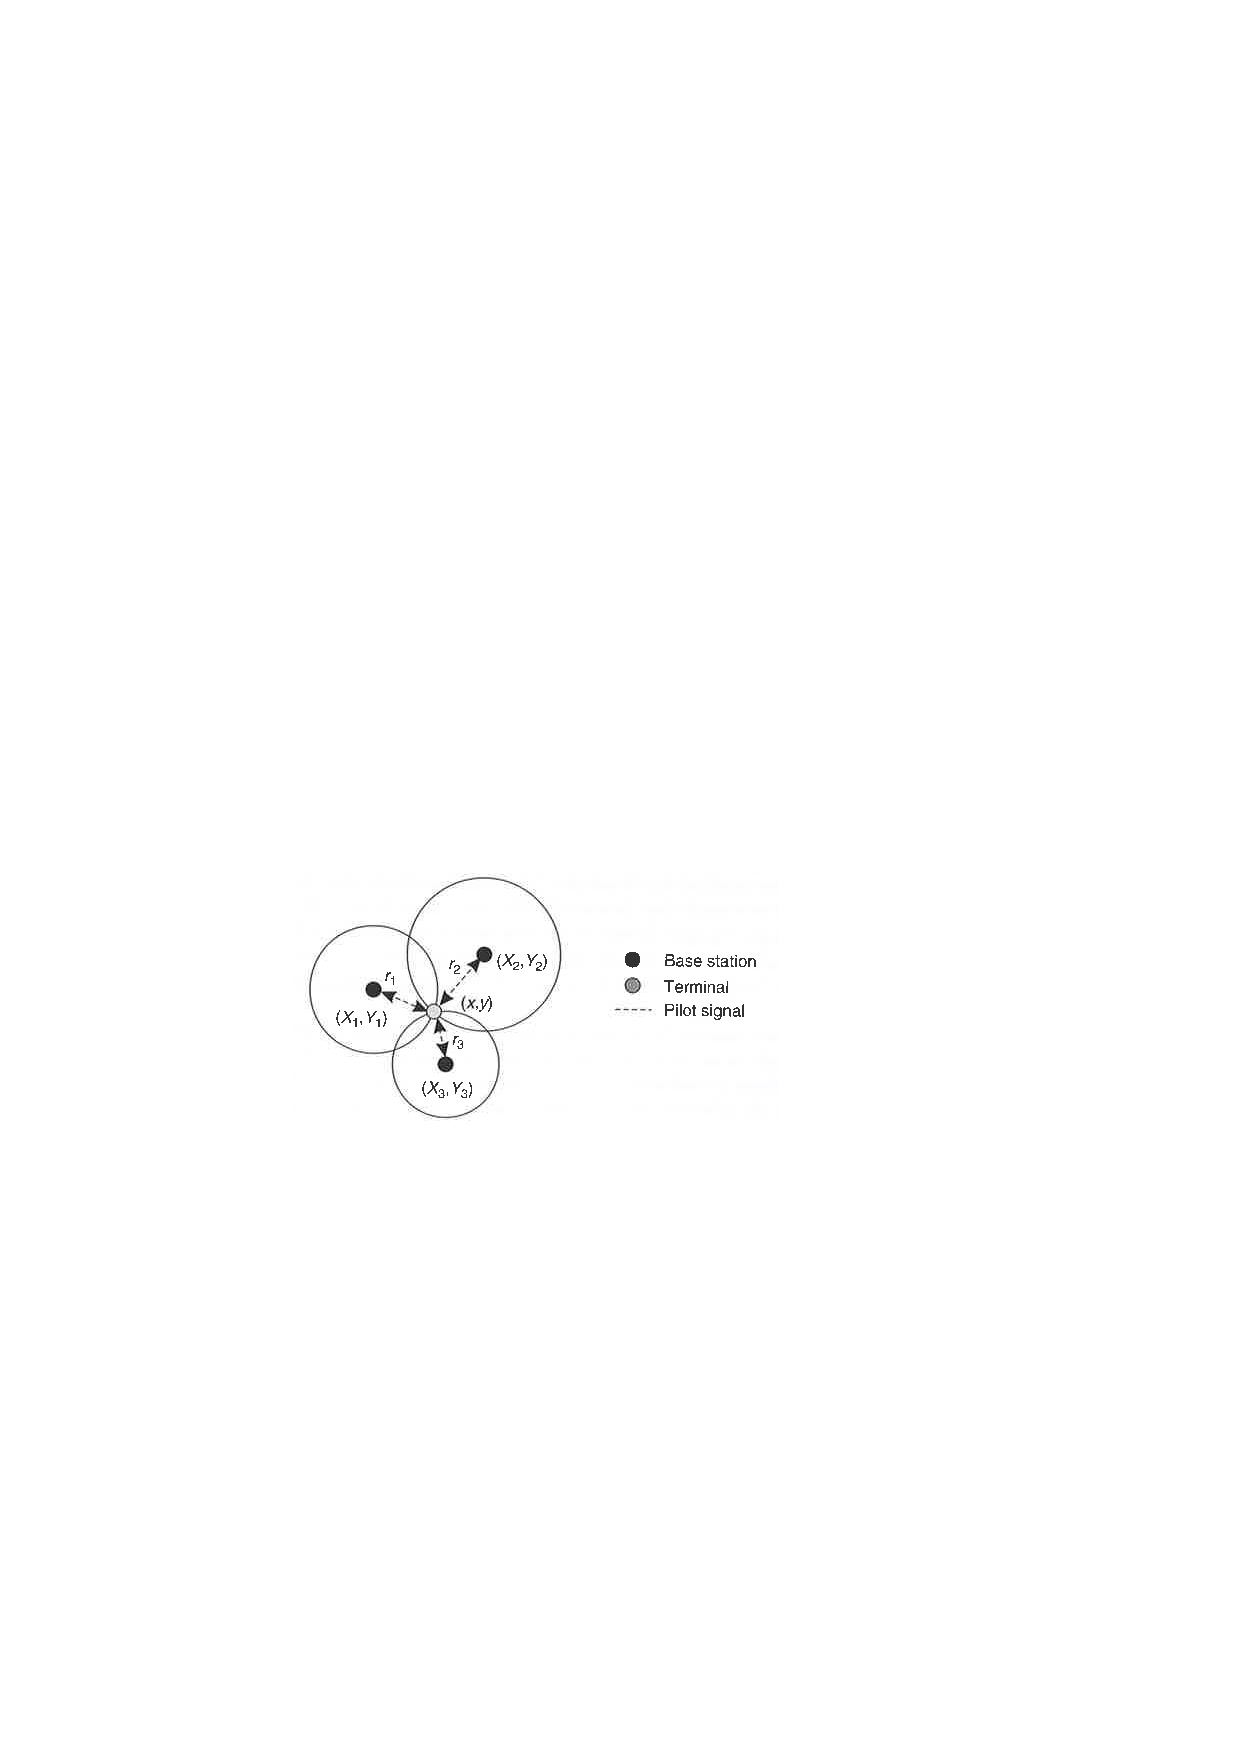
\includegraphics[width=0.7\textwidth]{circular_lateration.pdf}
    \caption{Circular lateration with three base stations \cite{kupper2005location}}
    \label{fig:circular_lateration}
\end{figure}

In three-dimensional space, each distance measurement defines a sphere around a base station. 
Kolodziej and Hjelm \cite{kolodziej2017local} note that with only three base stations, the target's position is narrowed down to two possible points where the spheres intersect. 
Typically, one of these points can be dismissed as implausible, such as a location in outer space. 
To eliminate any ambiguity, a fourth base station is introduced, ensuring a unique position fix. Additionally, the fourth base station aids in synchronizing clocks.

\subsubsection{Hyperbolic Lateration}
In contrast to circular lateration, hyperbolic lateration determines a position by measuring differences in distance rather than absolute distances. A hyperbola represents all points that maintain a constant range difference relative to two fixed points, typically two base stations. K\"upper \cite{kupper2005location} explains that with the known range difference between the target and two base stations, the target's possible locations are constrained along a hyperbolic path between them. This method, illustrated in part (a) of Fig.~\ref{fig:hyperbolic_lateration}, uses two base stations to determine a single hyperbolic path. However, with just two base stations, the target's precise location cannot be unambiguously determined, as it could lie anywhere along the hyperbola.
To resolve this ambiguity, a third base station is introduced, as shown in (b). By adding this third base station, a second hyperbola is created and the target's position is estimated at the intersection of these two hyperbolas. In three-dimensional space, the principle extends to hyperboloids, requiring at least three base stations for an unambiguous position fix. A key advantage of hyperbolic lateration is that it only requires synchronization among the base stations' clocks, rather than between the stations and the target, simplifying timing coordination.

\begin{figure}[htbp]
    \centering
    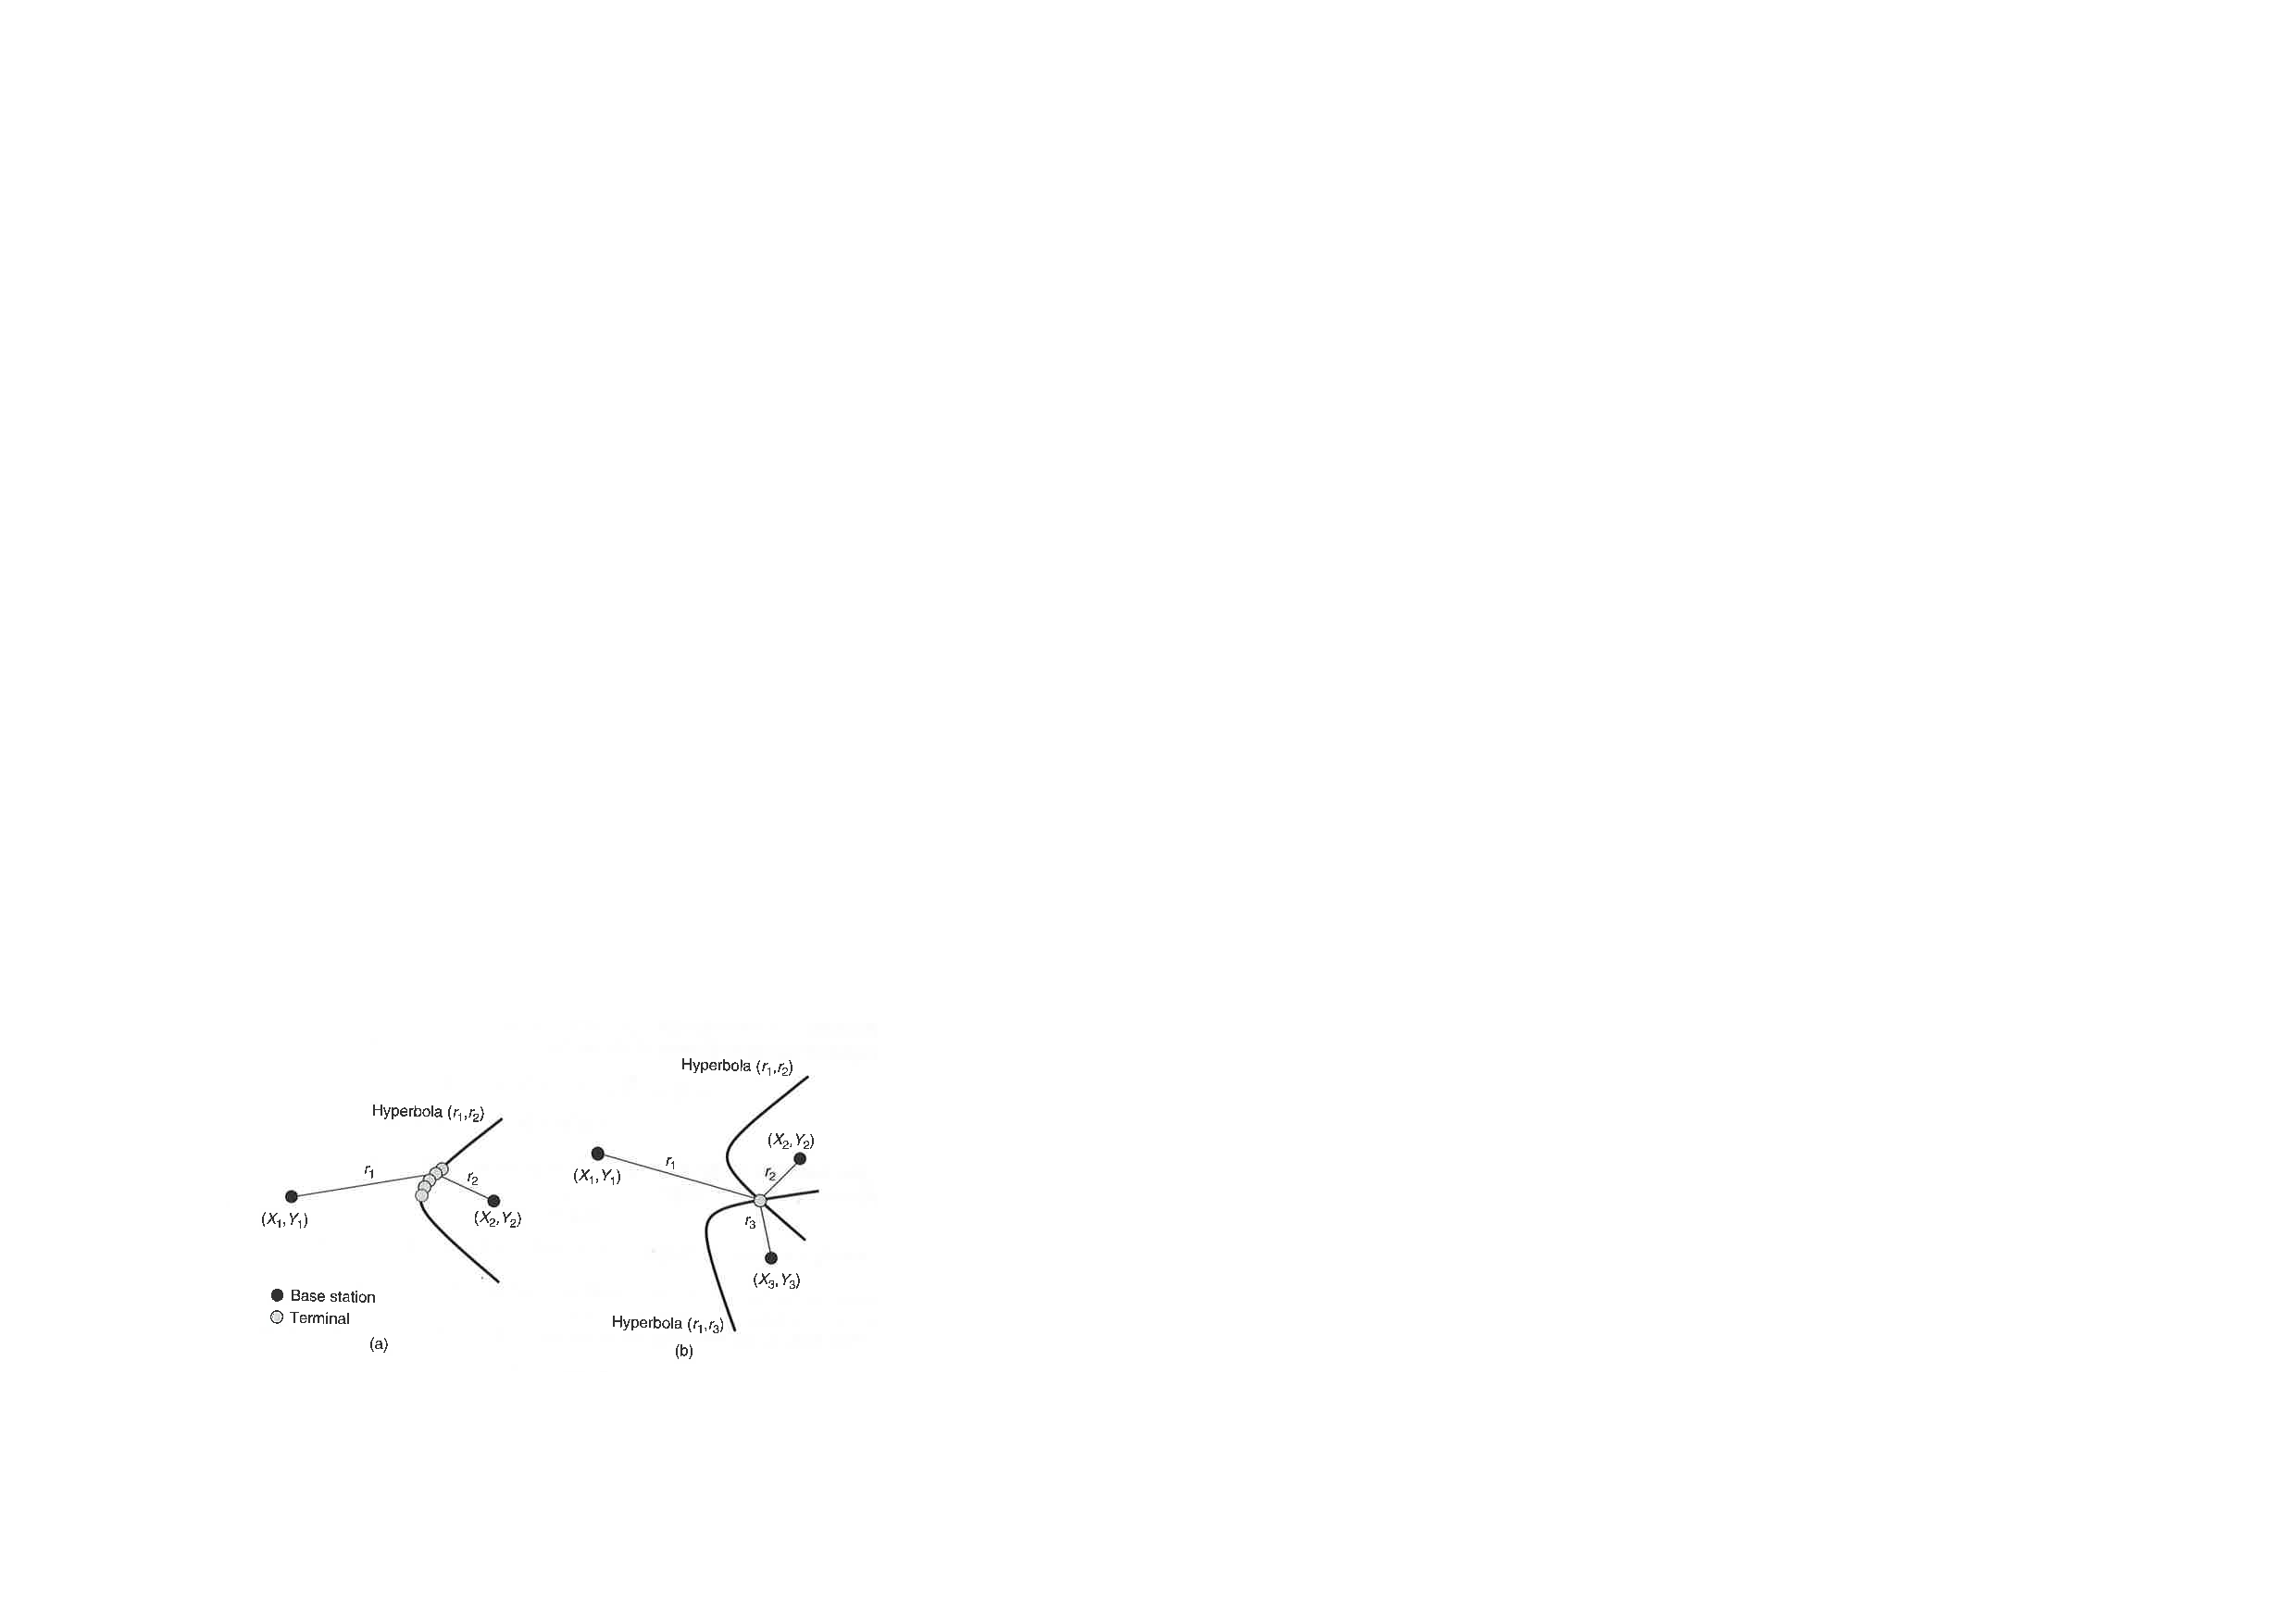
\includegraphics[width=0.7\textwidth]{hyperbolic_lateration.pdf}
    \caption{Hyperbolic lateration with two (a) and three (b) base stations \cite{kupper2005location}}
    \label{fig:hyperbolic_lateration}
\end{figure}


\subsection{Angulation}
Angulation is a positioning technique that determines an object's location based on the angles at which signals are received from multiple reference points, rather than measuring distances. According to K\"upper \cite{kupper2005location} it is also called Angle of Arrival (AoA) or Direction of Arrival (DoA). Werner \cite{werner2014indoor} explains that by using directional antennas or other angle-measuring equipment, the system identifies the direction of incoming signals from known base stations or access points. Once the angles from at least two base stations are known, the object's position can be triangulated by drawing lines along these angles, the point where the lines intersect reveals the target's location, as shown in Fig.~\ref{fig:angulation2}.

\begin{figure}[htbp]
    \centering
    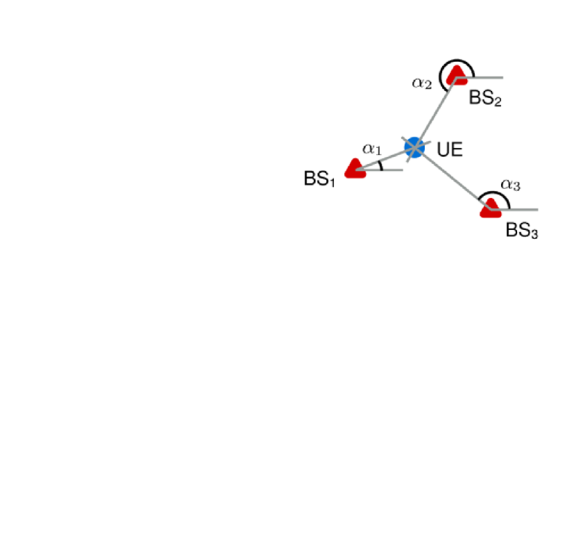
\includegraphics[width=0.4\textwidth]{angulation2.pdf}
    \caption{Triangulation \cite{militaru2024positioning}}
    \label{fig:angulation2}
\end{figure}

In three-dimensional space, a third angle may be required for accurate positioning. Angulation offers an effective alternative to lateration methods, particularly in environments where measuring precise distances is challenging due to signal reflections or interference. However, it does require precise angle measurements, which can be sensitive to minor errors in directionality, especially at long distances.

\subsection{Pattern Matching}
\subsection{Inertial Navigation}
Inertial navigation approximately calculates the current position by starting from a known location and using measurements of direction, velocity and time to compute the path traveled.
When the calculated path is then compared to an initial point of reference, the position can be determined. 
This method represents a modern approach to dead reckoning, which was widely used by European explorers during the Middle Ages. 
They navigated using tools such as compasses, log lines and estimates of speed and time, as detailed by Taylor \cite{taylor1950deadreckoning}. 
Figure~\ref{fig:deadreckoning} illustrates this process of approximating position through dead reckoning.

\begin{figure}[htbp] 
    \centering 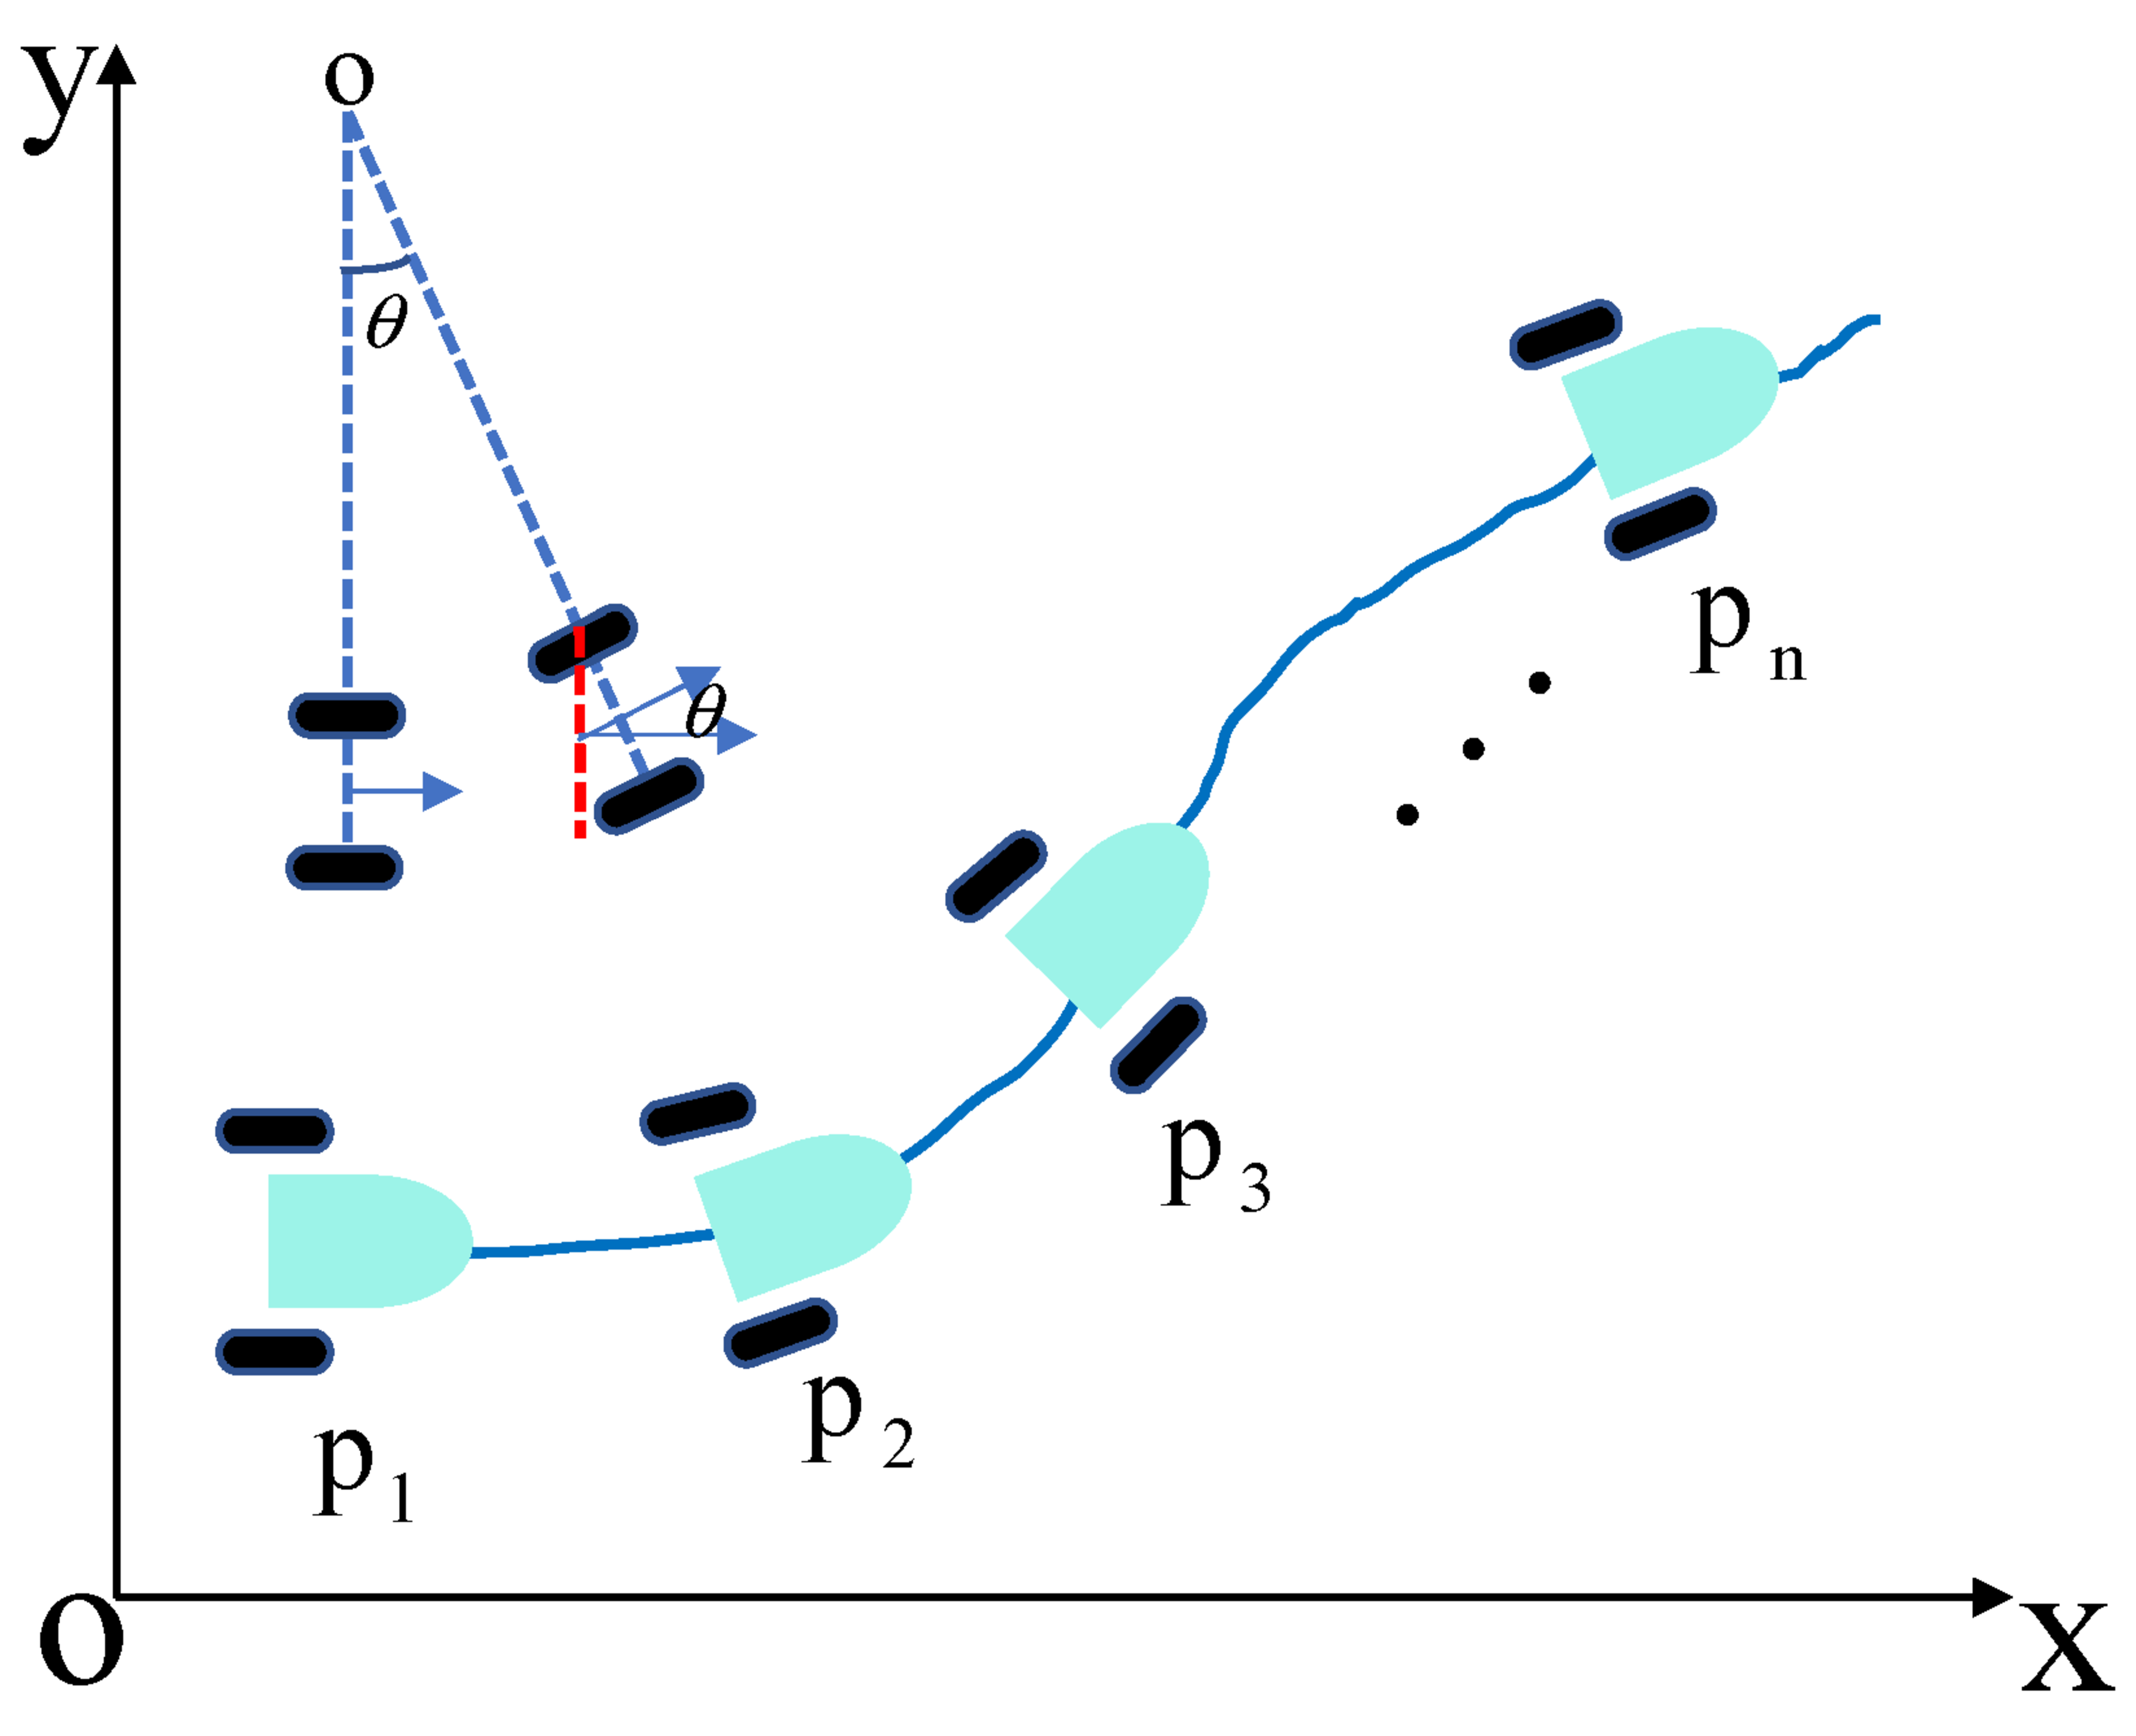
\includegraphics[width=0.5\textwidth]{deadreckoning.pdf} 
    \caption{Dead Reckoning \cite{wei2022positioning}} 
    \label{fig:deadreckoning} 
\end{figure}

While inertial navigation shares these conceptual roots, it leverages modern technology to measure motion far more precisely. 
An Inertial Navigation System (INS) relies on data from an Inertial Measurement Unit (IMU), which contains accelerometers to measure linear acceleration and gyroscopes to track angular rotation. 
Once an initial position is established using methods like lateration or angulation, an INS operates independently and doesn't rely on external electromagnetic signals like satellites or radio signals. 
This self-contained nature makes inertial navigation highly robust against signal obstructions and manipulation, unlike GNSS systems, which can suffer from signal disruptions in certain environments. 
Urban canyons, mountain valleys, and tunnels can create radio shadows that block satellite signals as per Zhang et al. \cite{zhang2021gnss}. 
Furthermore, as Enge \cite{enge1994global} and Ruegamer et al. \cite{ruegamer2015jamming} highlight, GNSS is vulnerable to jamming, where interference blocks satellite signals, and spoofing, where fake signals deceive receivers into showing incorrect positions or times.
In such scenarios, measurements from inertial sensors can be used as an enhancement for GNSS systems, but they still are highly susceptible to errors.
El-Sheimy \cite{sheimy2006ins} explains that position errors grow quadratically as a result of velocity errors that stem from biases or inaccuracies in accelerometer measurements during the initial integration process. 
He further points out that errors in gyroscopic data are even more impactful, as they first produce angular inaccuracies, which then propagate into velocity errors that grow quadratically and ultimately result in cubic error in position. 
These errors can accumulate over time due to the lack of external reference points. 
To mitigate this, inertial navigation is often only applied in short-term uses, such as to bridge periods when line-of-sight to satellites is obstructed or to refine position fixes determined by GNSS systems. 
By combining the last known location obtained via GNSS with measurements captured by an IMU chip, a vehicle's movement can still be tracked during GNSS outages, e.g. driving through a tunnel.

% Brossard et al. \cite{brossard2020imu} explain that while Global Navigation Satellite Systems (GNSS) are the most reliable method for determining a position fix anywhere in the world, they can suffer from signal disruptions in certain environments. 
% Urban canyons, mountain valleys and tunnels can create radio shadows that block satellite signals as per Zhang et al. \cite{zhang2021gnss}. 
% Furthermore, as Enge \cite{enge1994global} and Ruegamer et al. \cite{ruegamer2015jamming} highlight, GNSS is vulnerable to jamming, where interference blocks satellite signals, and spoofing, where fake signals deceive receivers into showing incorrect positions or times.
% In such scenarios, Inertial Navigation Systems (INS) provide a valuable alternative. 
% Unlike GNSS, inertial navigation operates independently of external signals, making it robust against signal obstructions and manipulation. 
% INS estimates the current position by starting from a known location and using measurements of direction, velocity and time to compute the likely path traveled. 
% The initial position is typically established using more reliable methods like lateration or angulation.

% Inertial navigation is grounded in Newtonian mechanics, particularly Newton's first law of motion. 
% According to NASA \cite{nasa_newton_laws}, an object in motion continues in a straight line at constant speed unless acted upon by an unbalanced force. 
% This principle forms the basis for calculating an object's trajectory. 
% As Grewal et al. \cite{grewal2007global} explain, "the fundamental idea for inertial navigation […] comes from high-school physics: the second integral of acceleration is position." 
% In practical terms, this means that by measuring acceleration over time, integrating it to calculate velocity, and then integrating the velocity to calculate the distance traveled, position can be determined. 
% However, to accurately track position in three dimensions, additional data is required to account for turns and non-linear movements.
% This navigation method with ancient origins is known as dead reckoning and was widely used by European explorers during the Middle Ages. They navigated using tools such as compasses, log lines and estimates of speed and time, as detailed by Taylor \cite{taylor1950deadreckoning}.
% Figure~\ref{fig:deadreckoning} illustrates this process of estimating position through dead reckoning.

% \begin{figure}[htbp] 
%     \centering 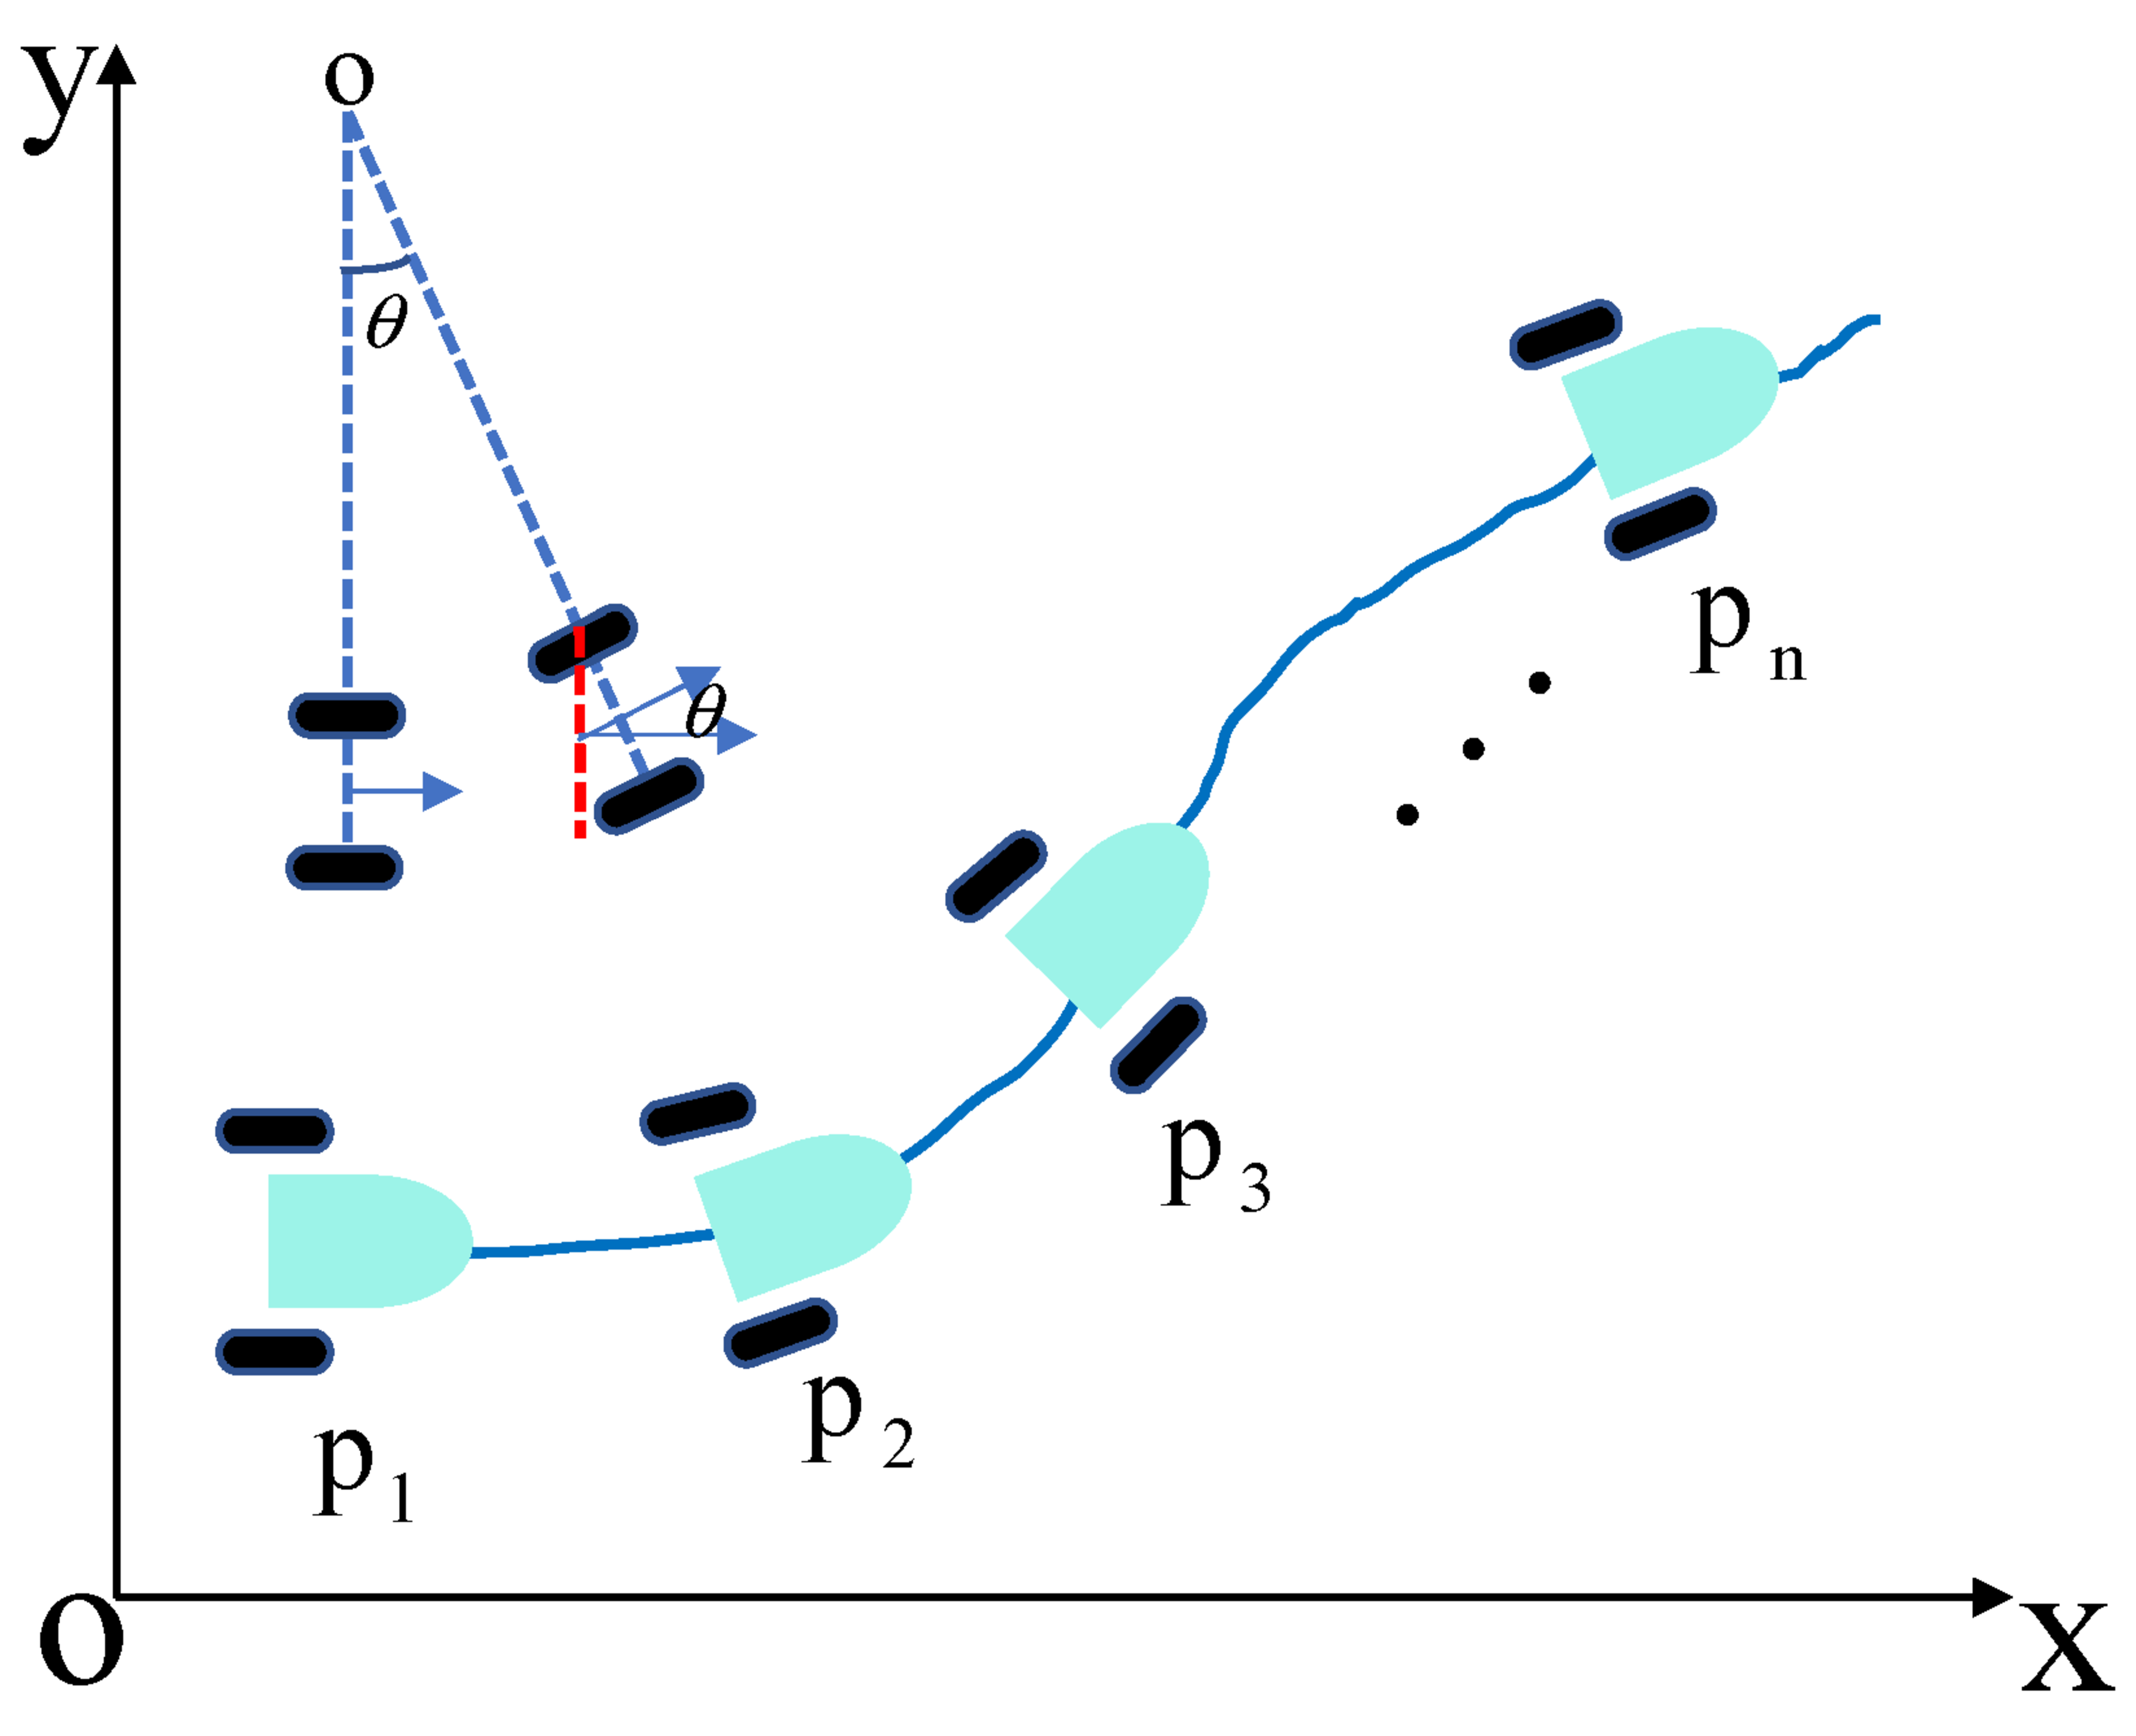
\includegraphics[width=0.5\textwidth]{deadreckoning.pdf} 
%     \caption{Dead Reckoning \cite{wei2022positioning}} 
%     \label{fig:deadreckoning} 
% \end{figure}

% While inertial navigation shares these conceptual roots, it leverages modern technology to measure motion far more precisely. 
% An INS relies on data from an Inertial Measurement Unit (IMU), which contains accelerometers to measure linear acceleration and gyroscopes to track angular rotation. 
% When an IMU's measurements are combined, they can reliably calculate a vehicle's position and orientation. 
% For instance, when a vehicle is traveling through a tunnel, GNSS signals are momentarily unavailable. 
% By combining the last known location obtained via GNSS with measurements captured by an IMU chip, a vehicle's movement can still be tracked during the GNSS outage, often with centimeter-level accuracy.
% Despite its advantages, INS has limitations, such as error accumulation over time due to the lack of external reference points, leading to drift in position estimates.
% To mitigate this, low-cost IMUs are primarily used to bridge periods when line-of-sight to satellites is obstructed.

% Inertial sensors are well suited for integration with GNSS systems owing to their
% complementary features.
% Unlike GNSS systems, the inertial navigation systems (INS) are self-contained and their
% performance is not degraded in environment as urban canyons, being independent of
% external electro-magnetic signals. Moreover INS are more accurate in the short term and
% they can supply data continuously with very high rate (at several hundred Hz, whereas
% GNSS receivers typically updates position and velocity at 1 to 20 Hz); INS can also
% provide attitude information.
% The main drawback of an INS is the degradation of its performance with time; in order
% to bound the errors to an acceptable level, regular updates are necessary and GNSS
% measurements can be used to this purpose.

\section{Positioning Systems}
\subsection{Cellular Positioning}
\subsection{GNSS}
%lee2014localization
%accuracy of GPS data is relatively low (more than 10m)
%winters2008travel
%The GPS system is a constellation of 24 satellites that broadcast data that can be processed by end-user devices to calculate their position using the Time of Arrival (TOA) method and applying circular lateration in combination with timing measurements. The constellation consists of six orbits spaced 60 degrees apart, with four satellites per orbit. This guarantees that a GPS receiver is under the coverage of at least four satellites at any given point in the earth’s surface.
%since the GPS transmissions from the satellites are very weak, the device must have a clear view of the sky to receive the transmissions used to calculate its position. This means that pure GPS positioning solutions do not work indoors or in situations where radio signals may be interrupted, such as during severe weather or in “urban canyons” (areas surrounded by many tall buildings)

\subsection{WLAN and Bluetooth Positioning}
\subsection{Inertial Navigation Systems}
% An Inertial Navigation System (INS) is a combination of sensors able to determine all
% navigation states of a moving object, i.e. position, velocity and attitude; the ensemble of
% sensors is an Inertial Measurement Unit (IMU) and consists of three accelerometers and
% three gyroscopes mounted on an orthogonal triad.
% To obtain the velocity of the moving object, the measured specific force should be
% corrected of the gravitational term, integrated once and the result added to the initial
% velocity. Integrating the obtained velocity and adding the initial position, yields the final
% position. So an INS can be considered a sophisticated Dead Reckoning (DR) system
% (El-Sheimy 2004). However the INS is actually more complicated because the measured
% specific force is expressed in a frame different from the frame in which velocity and
% position are usually expressed (navigation frame). For this reason the gyro triad is
% included in the IMU: gyros are able to measure angular rate with respect to the inertial
% frame, which, when integrated, provides the angular change with respect to the
% previous, supposed known, initial orientation. So gyros are used to transform the
% measured specific force in the navigation frame; the transformation can be mechanic,
% i.e. the IMU is physically aligned to the navigation frame (Gimbaled configuration), or
% analytic, i.e. the acceleration measurements are numerically transformed in the
% navigation frame (Strapdown configuration). Strapdown configuration is currently the
% more common strategy and is used in this work.
% An uncompensated error in the accelerometer measurement (e.g. a bias) is integrated
% once introducing a linear error in velocity, which in turn integrated will introduce a
% quadratic error in position (El-Sheimy 2004). The presence of an uncompensated gyro
% error is more critical, introducing linear error in angles and in turn yielding quadratic
% error in velocity and cubic error in position. Thus the INS performance strongly
% depends on the quality of the included gyros (El-Sheimy 2004).

% Another advantage of INS, as noted by Angrisano \cite{angrisano2010gnss}, is its ability to provide data at a high rate, often reaching several hundred Hertz. 
% Whereas GNSS receivers typically update position and velocity at rates ranging from 1 to 20 Hz. 
% Additionally, INS can supply attitude information.
% As noted by Angrisano \cite{angrisano2010gnss}, an INS is capable of providing data at high frequencies, often reaching several hundred Hertz, whereas GNSS receivers generally update position and velocity at rates ranging from 1 to 20 Hz. Additionally, an INS can supply attitude information.


% GNSS INS with MEMS (AI-based algorithm instead of traditional Kalman filter)
% The recent advances in MEMS technology has made possible the development of a
% generation of low cost inertial sensors, characterized by small size and light weight
% which represent an attractive option for commercial applications as pedestrian and
% vehicular navigation. MEMS-based INS are characterized by low performance too, so
% their use as part of an integrated navigation system is currently under investigation.
% Inertial navigation systems (INS) are a continuously running dead reckoning process and work independently from the outside world, which means that they don't rely on external signals like satellites or radio signals. 
% This closed-system property makes them ideal in situations where GNSS tracking or other external positioning systems are unavailable. 
% As stated by Brossard et al. \cite{brossard2020imu}, GNSS can lose signal in tunnels or crowded areas, is vulnerable to jamming and may not always give accurate or reliable location data.
%A six-axis IMU contains three accelerometers and three gyroscopes
%brossard2020imu
% High precision aerial or military inertial navigation systems
% achieve very small localization errors but are too costly for
% consumer vehicles. By contrast, low and medium-cost IMUs
% suffer from errors such as scale factor, axis misalignment and
% random walk noise, resulting in rapid localization drift [21]. This
% makes the IMU-based positioning unsuitable, even during short
% periods.
% Note that Global
% Navigation Satellite System (GNSS) allows for global position
% estimation but it suffers from phase tracking loss in densely
% built-up areas or through tunnels, is sensitive to jamming, and
% may not be used to provide continuous accurate and robust
% localization information, as exemplified by a GPS outage in the
% well known KITTI dataset [3], see Fig. 1.
%
% In INS, the Inertial Measurement Unit (IMU) can measure the three-axis angular velocities and three-axis accelerations of the current vehicle and calculate the speed and position of the object in the navigation coordinate system. It will not be affected by signal transmission and has high stability.

\subsection{Hybrid Systems}
